\chapter{Nonconvex optimal control problems with $L^q$ penalizations}

	
	\section{Penalties of the form $\int_{\om}|u|^q$ with $q\in [0,1)$}
		Optimal control problems with nonconvex $L^q$-quasinorms (with $q \in (0,1)$) can be regarded as a regularization of the so called $L^0$ sparse penalized problems, in which the optimal control fulfills a minimal support's volume criterion, promoted by the $L^0$ penalizer, see \cite{ito-kunisch2014, wachsmuth2011}.  However, depending on the regulization parameters present in the cost function,optimal controls induced by the  $L^q$-quasinorm entail subtle jump discontinuities and sparse properties that differs from those optimal controls generated by the $L^0$-pseudo norm; for instance, $L^q$ optimal controls may have smaller supports and, moreover, jump discontinuities may be not monotone, see Figure \ref{fig:jump}. These properties are relevant for optimal control as they enhance the sparsity and jump discontinuities characterization of the optimal controls.
	
	Optimal controls induced by $L^q$-quasinorm penalizers share similarities with those induced by $L^1$-norm and by the $L^0$ penalizer. It is well known that these controls tend to have small supports depending on the sparse regularization cost \cite{stadler2006}. However, a simple but essential difference in considering $L^q$-quasinorms is that jump discontinuities appear at the boundary of optimal control's support. This feature is potentially advantageous in several applications. 
	In particular, the sparsification effect induced by these penalizers are useful in applications requiring a sharp localized action of the control within the domain, which is crucial for instance, to reduce the cost of the tracking term, see \cite{casas}.  Other examples arising from inverse sparse reconstruction problems and image-processing-related applications can benefit from solutions with jump discontinuities. For instance, in imaging, the so called $TV^q$ penalizer enforces certain graphical features. 
	
	
 	Research on optimal control problems with $L^q$-quasinorm penalizers is recent.  Perhaps, the biggest recognizable difficulty in considering the $L^q$-quasinorm is the lack of convexity (a fortiori, the lack of weak lower semicontinuity) of the penalizer. Therefore, analyzing the existence of a solution such as developing efficient numerical algorithms are challenging tasks. In \cite{ito-kunisch2014}, the $L^0$ penalization was studied along with the $L^q$-quasinorm penalizer. In the last case,  a penalty given by the $L^2$-norm of the gradient was added to the cost, which allows compactness arguments to guarantee the existence of solutions in $H^{1}$. However, the gradient cost term removes the jump discontinuities from solutions, which is a relevant feature of the $L^q$-quasinorm. 
	
	The associated optimality conditions were derived in \cite{ito-kunisch2014} utilizing a $\rm{C}^1$ regularization of the nonconvex term. Furthermore,  \cite{merino2019} derived an optimality system by regularizing the cost with a continuous nonconvexity, and thereafter, the subsequent application of the difference-of-convex programming, including control constraints in the case of linear elliptic second-order PDEs. In both cases, the optimality conditions depend on a regularization parameter that is taken to a limit to characterize the optimality conditions of the original problem.
	
 	
In this paper, we investigate an optimal control problem subject to a linear second-order elliptic partial differential equation.	The cost function  $J: L^2(\om) \times (\om) \to \reals$ involving an $L^q$--quasinorm ($q\in (0,1)$) penalization, is given by
	\begin{equation}\label{eq:cost_q}
		\displaystyle J{(y,u)}= ~\frac{1}{2}\| y-y_d \|^2_{L^2(\om)}+\frac{ \alpha}{2}\|u\|^2_{L^2(\om)}+\beta \int_\om |u|^{q} dx.
	\end{equation}

We formulate the following distributed optimal control problem using the objective functional \eqref{eq:cost_q} as follows:
	\begin{equation}
		\tag{$P$} \label{eq:OCP}
		\begin{cases}
			\displaystyle\min_{(y,u)} J(y,u)\\
			\hbox{ subject to: }\\
			\hspace{40pt}\begin{array}{rll}
				A y=&u + f, &\hbox{in  } \om, \\
				y=&0, &\hbox{on  }  \Gamma.
			\end{array}			
		\end{cases}
	\end{equation}
	In our setting, $\om \subset \reals^n$ is a bounded Lipschitz domain, and $y_d$ and $f$ are given functions in $L^2(\om)$.
	Moreover, $A$ is a uniformly elliptic second--order differential operator of the form:
	\begin{equation}\label{eq:A}
		(Ay) (x) = - \sum_{i,j=1}^n \frac{\partial}{\partial x_i}	\l( a_{ij}(x)\frac{\partial y(x)} {\partial x_j }\r) +c_0 y(x),
	\end{equation}
	%
	with coefficients $a_{ij}$ in $\rm{C}^{0,1}(\bar\om)$, and $c_0\geq 0$ in $L^{\infty}(\om)$. In addition, the matrix $(a_{ij})$ is symmetric and fulfills the uniform ellipticity condition: 
	\begin{equation}\label{eq:uelliptic}
		\exists\, \sigma>0 : \quad   \sum_{i,j=1}^n a_{ij}(x) \xi_i\xi_j \geq \sigma |\xi|^2, \quad \forall \xi \in \reals^n, \text{for almost all } x \in \om. 	
	\end{equation}  	

	
	\emph{Our contribution.} Here, we highlight the key contributions of this paper.
	\begin{itemize}
		\item We proved the existence of (generalized) optimal controls  $L^2$ for the $L^q$-quasinormed ($q\in(0,1)$) optimal control problems, by defining a thresholding operator, and extending the result for $L^0$-pseudonorm penalized optimal controls given by Ito and Kunisch \cite{ito-kunisch2014}.
		%\item We provide a novel approximation result for the solutions of $L^q$-quasinorm optimal controls to $L^0$-pseudonorm optimal controls in terms of $\|\bar u_0 - \bar u_q\|_{L^2(\om)}$.
		\item We introduced a \emph{Sequential Quadratic Hamiltonian} method (SQH) for solving \eqref{eq:OCP}, satisfying hypotheses for convergence.
		\item We provide an error analysis for the variational discretization approach using the finite-element method for problem \eqref{eq:OCP}. 
  \item We develope some numerical tests illustrating the associated theory.
	\end{itemize}
	 	
	
	\emph{Organization of the paper.}  We begin by deriving an optimality system in Section 2, for which we analyze its solvability and, subsequently, deduce the existence of the optimal controls. The box-constrained case is briefly discussed at the end of this section. In section 3, we formulate the \emph{Sequential Quadratic Hamiltonian} method for solving the optimal control problem.  We show the algorithm's performance thorough numerical tests. Section 4 is devoted to the variational finite-element approximation of the optimal control problem. Several convergence results and error estimates are discussed. This analysis is followed by several numerical experiments aiming to provide insight into the approximation behavior of the solutions. Finally, we draw conclusions from our findings.
	
	
	\section{Existence of solution and optimality conditions }
    \section{Problem formulation}
    \section{Partial convexification of the $L^q$ terms}
    \section{ The Maximum Principle and its equivalence with the Partial convexification of the problem}
    \section{Incoporating control constrains}
    \section{Incorporating mixed control-state cosntrains}
    
	We argue for the existence of a solution to problem \eqref{eq:OCP}, following the methodology presented in \cite{ito-kunisch2014}, where the authors demonstrated the existence of a solution using the $L^0$-pseudonorm as a penalizer in the cost function. We proceed by first deriving the first-order necessary optimality conditions that characterize solutions to \eqref{eq:OCP}. Then, after obtaining a solution to these conditions, we will verify that it is, indeed, a global minimum for \eqref{eq:OCP}.

We denote by $a(\cdot, \cdot):H_{0}^{1}(\om) \times H_{0}^{1}(\om)\to \reals$  the bilinear form associated to the second-order differential operator $A$, defined by $$a(y,v)=\int_\om a_{ij}(x)\frac{\partial y(x)}{\partial x_i} \frac{\partial v(x)}{\partial x_i} dx + \int_\om c_0(x)\,y(x)v(x)\,dx, $$
while $a^*$ denotes the corresponding bilinear operator associated to $A^*$.
	
	Thanks to the Lax--Milgram theorem and the elliptic regularity \cite{brezis2010}, we know that for every $w \in L^2(\om)$ there exist $y\in H_{0}^{1}(\om)$ and a positive constant $c_a>0$, satisfying: 
	\begin{subequations}\label{eq:state_formul}
		\begin{align}
			&a(y,v) = (w,v)_{L^2(\om)}, \quad \forall v \in H_{0}^{1}(\om),\label{eq:state}\\
			&\norm{y}_{H_{0}^{1}(\om)} \leq c_a\norm{w}_{L^2(\om)}. \label{eq:state_continuity}
		\end{align}
	\end{subequations}
 The same is true for the adjoint problem:
	\begin{subequations}
		\begin{align}
			&a^*(z,v) = (w,v)_{L^2(\om)}, \quad \forall v \in H_{0}^{1}(\om),\label{eq:state*}\\
			&\norm{z}_{H_{0}^{1}(\om)} \leq c_a^*\norm{w}_{L^2(\om)}\label{eq:esti_state*}.
		\end{align}
	\end{subequations}
for some positive constant $c_a^*$.

Furthermore, thanks to Theorem 4.4 in \cite{stampacchia1965} and the continuous injection $L^2(\om) \hookrightarrow W^{-1,p}(\om)$, we have that, for a fixed $p>n$, there exists a linear and continuous operator $S:L^2(\om)\to L^{\infty}(\om)\cap H_{0}^{1}(\om)$, which assigns any $w\in L^2(\om)$  the corresponding state $y$  satisfying \eqref{eq:state} with $w$ as right-hand side. The continuity of $S$ also implies the existence of a constant $c_{\infty}>0$ such that the solution $y=Sw$ of \eqref{eq:state} satisfies
\begin{equation}\label{eq:esti_state_uniform}
    \norm{y}_{L^{\infty}(\om)}\le c_{\infty}\norm{w}_{L^2(\om),}
\end{equation}
Analogously, for the solution $z$ of \eqref{eq:state*} it holds that 
\begin{equation}\label{eq:esti_state*_uniform}
    \norm{z}_{L^{\infty}(\om)}\le c_{\infty}\norm{w}_{L^2(\om),}
\end{equation}
for some constant $c_{\infty}^*>0$. We denote by $S^*:L^2(\om)\to L^{\infty}(\om)\cap H_{0}^{1}(\om)$ the corresponding solution operator that for any $w\in L^2(\om)$ assigns the  solution $z=S^*(w)$ of \eqref{eq:state*}.

	\subsection{Optimality conditions}	
	
	
	The adjoint state is an essential tool to represent optimality conditions. Given a control $u \in L^2(\om)$ with associated state $y\in H_{0}^{1}(\om)$, we introduce the adjoint state $\varphi$ as the solution of the following variational problem, which can be in the same way as problem \eqref{eq:state}: 
	\begin{align}\label{eq:costate}
		&a^*(\varphi,v) = (y_d-y,v)_{L^2(\om)}, \quad \forall v \in H_{0}^{1}(\om)
	\end{align}	
	
	We define the Hamiltonian associated with the optimal control \eqref{eq:OCP} problem as follows:
	\begin{equation} \label{eq:Hamiltonian}
    \mathcal{H}(x,y,u,p):=\frac12 |y-y_d|^2+\frac{\alpha}{2}u^2 + \beta |u|^q + p u.
    \end{equation}
	
	We apply Theorem 2.2 in \cite{ito-kunisch2014} by choosing $\ell(x,y(x))=\frac{1}{2}(y(x)-y_d)^2$, $h(u)=\frac{\alpha}{2}|u|^2+\beta|u|^q$, $f(\cdot,y,u(\cdot))=u(\cdot)$, $\langle Ey,\cdot\rangle_{X^*,X}=a(y,\cdot)$ and $X=H_{0}^{1}(\om)$. This setting verifies the hypothesis of \cite[Theorem 2.2]{ito-kunisch2014}; therefore,  if $(\bar y, \bar u)$ is a solution of  \eqref{eq:OCP}, and $\varphi$ is the associated adjoint state, we conclude that for almost all $x \in \om$ it holds: 
	$$
		\mathcal{H}(x,\bar y(x),\bar u(x),\varphi (x))\leq \mathcal{H}(x,\bar y(x),u,\varphi (x)),
	$$
	 for all $u \in \reals$ and almost all $x\in\om$. 
	 
	 Writing the last relation explicitly we find that $\bar u(x)$ satisfies
	\begin{equation}\label{eq:fonc_H}
		\frac{\alpha}{2}\bar u(x)^2 + \beta |\bar u(x)|^q + \varphi(x) \bar u(x) \leq \frac{\alpha}{2}u^2 + \beta |u|^q + \varphi(x) u
	\end{equation}
	for almost all $x$ and all $u\in \reals$. 
	
	Taking into account \eqref{eq:fonc_H}, we seek to characterize $\bar u(x)$ for almost all $x\in \om$ by studying the following one-dimensional problem:
	\begin{equation}\label{eq:1dlq}
		\bar u \displaystyle\in  \argmin_{u\in \reals} \left\{g(u):= \frac{\alpha}{2}u^2+\beta |u|^q + pu \right\},
	\end{equation}
	where $p$ is a given real number.
	
	
	It is clear that if $\alpha>0$, then $g$ has at least one minimum, because it is continuous and coercive. First, let us consider the case where a minimum $\bar u \not =0$. Then, $g$ is differentiable and $\bar u$ satisfies the necessary condition 
	\begin{equation}\label{eq:1d_fonc}
		\alpha \bar u + \beta q |\bar u|^{q-1} \sign (\bar u) + p= 0. 	
	\end{equation}
	%
	Multiplying the last equality by $\bar u$ and replacing $p\bar u=-\alpha\bar u^2-\beta q |\bar u|^{q}$ in $g(\bar u)$, we have  that $\bar u$  satisfies the condition:
	
	$$ 
	  0=g(0)\geq g(\bar u) = \frac{\alpha}{2}\bar u^2 + \beta |\bar u|^{q} + p\bar u =  -\frac{\alpha}{2}\bar u^2 + \beta (1-q) |\bar u|^{q}.
	$$ 
Therefore, we deduce that
	\begin{equation}\label{eq:jump_bound}
		|\bar u| \geq \jump_q:=\l(2(1-q) \frac{\beta}{\alpha} \r)^{\frac{1}{2-q}}.
	\end{equation}
Thus, $|\bar u|$ is bounded away from 0 whenever it is not null, and $\jump_q$ estimates the jump discontinuity. Figure \ref{fig:jump} depicts the behavior of $\jump_q$ as a function of $q$ for fixed $\alpha$ and $\beta$. Here, we observe that for certain ratios $\beta/\alpha$ the convergence to $\jump_0=\sqrt{\frac{2\beta}{\alpha}}$ (when $q\to 0$), corresponding to the jump value of the $L^0$-pseudo norm is not monotone, and can reach larger values than $\sqrt{\frac{2\beta}{\alpha}}$.

\begin{figure}[ht!]
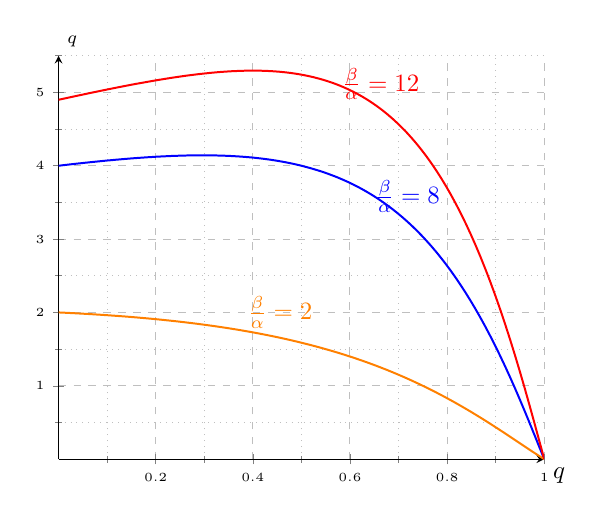
\begin{tikzpicture}[scale=0.9]
\begin{axis}[
    %title={Plot of $(2(x-1) \cdot 0.1)^{\frac{1}{2-x}}$ for $x$ in $[0,1]$},
    xlabel={$q$},
    ylabel={$\jump_q$},
    xmin=0, xmax=1,
    ymin=0, ymax=5.5, % Adjust the y-axis limits as necessary
    grid=both,
    minor tick num=1,
    major grid style={lightgray,dashed},
    minor grid style={lightgray,dotted},
    samples=100, % Increase for a smoother plot
    no marks,
    tick label style={font=\tiny},
    axis lines=middle,
    xlabel style={at={(ticklabel* cs:1)},anchor=north west}, % Adjust label position
    ylabel style={at={(ticklabel* cs:1)},anchor=south west} % Adjust label position
    ]
\addplot[blue, thick, domain=0:1] {(2*(1-x)*8)^(1/(2-x))} node[pos=0.3, above] {$\frac{\beta}{\alpha}=8$};
\addplot[orange, thick, domain=0:1] {(2*(1-x)*2)^(1/(2-x))} node[pos=0.25, above] {$\frac{\beta}{\alpha}=2$};
\addplot[red, thick, domain=0:1] {(2*(1-x)*12)^(1/(2-x))}node[pos=0.20, above] {$\frac{\beta}{\alpha}=12$};
\end{axis}
\end{tikzpicture}
\caption{Plot of the jump estimate  $\jump_q$ for different ratios $\beta/\alpha$. $\jump_0= \sqrt{2\beta/\alpha}$ at $q=0$ corresponds to $L^0$-pseudo norm penalizer}	
\label{fig:jump}
\end{figure}
	

\begin{lemma}\label{l:thresholds} Let $\bar u \not =0$ be a minimizer of $g$, i.e. $\bar u$ satisfies \eqref{eq:1dlq}. Then, it follows that
$$|\bar u| \geq \jump_q, \quad \text{if and only if, }\quad |p|\geq \omega_q ,$$
where $\omega_q=\l( 2(1-q) \alpha^{1-q}\beta \r)^{\frac{1}{2-q}} + \beta q \l(2(1-q) \frac{\beta}{\alpha} \r)^{\frac{q-1}{2-q}}$.
\end{lemma}
\begin{proof}
Without loss of generality, let us suppose that $\bar u >0$. The case $\bar u <0$ follows by symmetric arguments. Now,  let us compute the second derivative of $g$. By \eqref{eq:jump_bound} \textcolor{red}{No estoy seguro si la ecuación citada tiene algo que ver con la deducción de abajo. Entiendo, mas bien, que dado que $q<1$, $q-2<0$, por lo que la monotonía de la función $t\mapsto t^{q-2}$ implica que para $t>\jump_q/(2^{1/(2-q)})$, se tiene $\alpha-\beta 1(1-q)t^{q-2}>\alpha -\beta q(1-q)(\jump_q/(2^{1/(2-q)}))^{q-2}$},  we have that for $t>\jump_q/(2^{1/(2-q)})$ the second derivative is positive:
	$$
	g''(t)= \alpha -\beta q(1-q)  t^{q-2} > \alpha - \beta q(1-q)  \l(\frac{\jump_q}{2^{1/(2-q)}}\r)^{q-2} = \alpha - q\alpha >0,
	$$
showing that the function $t \mapsto \alpha t + \beta q t^{q-1}$ is strictly increasing for $t\geq\jump_q>\jump_q/(2^{1/(2-q)})$ \textcolor{red}{La monotonía se probó solo para $\jump_q/(2^{1/(2-q)})$}. Since $|\bar u|\geq \jump_q\textcolor{red}{>\jump_q/(2^{1/(2-q)})}$, we have
	\begin{align}
		|p| = \alpha |\bar u| + \beta q |\bar u|^{q-1}\geq & \alpha | \jump_q| + \beta q | \jump_q|^{q-1} \nonumber\\
		&=\l( 2(1-q) \alpha^{1-q}\beta \r)^{\frac{1}{2-q}} + \beta q \l(2(1-q) \frac{\beta}{\alpha} \r)^{\frac{q-1}{2-q}}=\omega_q,  \nonumber
	\end{align}
	%
 and conversely, if $|p|\geq w_q$, then the strictly monotonicity of $t \mapsto \alpha t + \beta q t^{q-1}$  implies that $|\bar u|\geq\jump_q$.
\end{proof}

 The threshold quantity $\omega_q$ can be used to characterize a global solution of \eqref{eq:1dlq} in terms of the size of  $p$. Indeed, we define $\bar u = \Phi_q(p)$ given by
	
	\begin{equation}\label{eq:PHI1}
		%
		\Phi_q (p) =	
		%
		\begin{cases}
			\argmin_{u} g(u), & \text{ if } |p| > \omega_q, \\
			0,                          &	 \text{ otherwise.}
		\end{cases}
	\end{equation}
		%
	\begin{remark}
	Equation \eqref{eq:PHI1} is semi-implicitly defined and, in practice, it has to be solved approximately. However, for the special cases $q=\frac12$ and $q=\frac23$, explicit solutions can be derived from the proximal mapping discussed in \cite{CaoZungXu2013}. Indeed, calculating the proximal of $|\cdot|^q$ we get:
	$$\text{\textnormal{prox}}_{|\cdot|^q,\frac{1}{\rho}}(t):=\argmin_{u} \l\{|u|^q+\frac{1}{2\rho}|u-t|^2 \r \},$$
that is equivalent to minimize $g$ defined in \eqref{eq:1dlq} for $\rho=\frac{2\beta}{\alpha}$. Thus, for $q=\frac12$, we have that $\varPhi_{\frac12}$ becomes:
		\begin{equation}\label{eq:PHI1 q=1/2}
		%
		\Phi_{\frac12} (p) =	
		%
		\begin{cases}
			\phantom{-}\frac23 |p|\big(1+\cos(\frac{2\pi-2 p_{\beta/\alpha} }{3})) \big), & \text{ if } p > \frac{54^{\frac13}}{4}\big(\frac{2\beta}{\alpha}\big)^{\frac23}, \\
			-\frac23 |p|\big(1+\cos(\frac{2\pi-2p_{\beta/\alpha}}{3})) \big), & \text{ if } p< -\frac{54^{\frac13}}{4}\big(\frac{2\beta}{\alpha}\big)^{\frac23}, \\
			\phantom{-}0,                          &	\text{ otherwise},
		\end{cases}
	\end{equation}
	with $p_{\beta/\alpha}=\arccos \Big(\frac{\beta}{4\alpha}\big(\frac{|p|}{3}\big)^{-\frac23}\Big)$.
\end{remark}	

	\begin{theorem}\label{t:monotone_phi}
		Given $p \in \reals$, $\Phi(p)$ is well defined, and $\bar u =\Phi(p)$ is a global solution for one-dimensional problem \eqref{eq:1dlq}.
	\end{theorem}
	
	\begin{proof}
		First, we consider the case $|p| \leq  \omega_q$. If $p=0$ is clear that $\bar u=0$ is a global solution for \eqref{eq:1dlq}. Let us prove that $\bar u =0$ is a global solution for \eqref{eq:1dlq} when $0<|p|\leq \omega_q$. Arguing by contradiction, suppose that $0 = \Phi(p)$ is not a global solution. Then, there is at least one point where the value of $g$ is below 0. By continuity and coercitivity of $g$, it reaches its minimum (without loss of generality) at some $\tilde u>0$ such that $g(\tilde u) <0$. Now, since $g$ is differentiable at $\tilde u$, it follows that 
		$$ 0 = g'(\tilde u) = \alpha \tilde u + \beta q (\tilde u)^{q-1} + p, $$		
		implying that  $$ 0 = g'(\tilde u)\tilde u = \alpha \tilde u^2 + \beta q (\tilde u)^{q} + p\tilde u = g(\tilde u) + \frac{\alpha}{2}\tilde u^2 + \beta (q-1) (\tilde u)^{q}. $$
		Considering that $g(\tilde u)<0$, we obtain that $\beta (1-q) (\tilde u)^{q}<\frac{\alpha}{2}\tilde u^2$ which in turn implies $\tilde u> \jump_q$. Thus, $p<-\omega_q$, \textcolor{blue}{accordingly to Lemma \ref{l:thresholds}}, contradicting that $|p|\leq \omega_q$. The same arguments apply by assuming that $\tilde u<0$.
		
		On the other hand, if $|p|>\omega_q$, we shall prove that $\bar u = \Phi(p)$ is well defined by showing that in this case, $g$ has only one minimum.  Again, without loss of generality, we assume that $p<-\omega_q$. By symmetry, the arguments are analogous for $p>\omega_q$. Since $\bar u$ minimizes $g$, then $g(\bar u) \leq g(\jump_q)$. Replacing $\jump_q= (2(1-q)\frac{\beta}{\alpha})^{\frac{1}{2-q}}$, we obtain 
		%
		\begin{align*}
			g (\bar u) \leq   g(\jump_q) <& \frac{\alpha}{2} {\jump_q}^2 + \beta {\jump_q}^{q} -\omega_q \jump_q\\
			=&-\frac{\alpha}{2} {\jump_q}^2 + \beta(1-q) {\jump_q}^{q} = \jump_q^2\left(-\frac{\alpha}{2}+\beta (1-q)\jump_q^{q-2}\right)=0.
		\end{align*} 
		Therefore, $g(\bar u)\textcolor{blue}{\le} g(\jump_q)\textcolor{blue}{<0}$. Moreover, since $p<-   \omega_q$ implies that $g(u)\geq 0$ for all $u\leq 0$, then $\bar u>0$. Furthermore, \textcolor{red}{since} $g$ is differentiable in $\reals^+$, then $\bar u$ must satisfy 
		
		\begin{equation}\label{eq:fonc_ell}
			\alpha \bar u + \beta q \textcolor{blue}{\bar u^{q-1}} = -p 
		\end{equation}
		
		The function \textcolor{blue}{$s(u):= \alpha   u + \beta q   u^{q-1} $ defined for all $u>0$} attains its minimum at $\hat u = \jump_q({q}/{2})^{\frac{1}{2-q}}$. In addition, it is strictly monotone increasing for all  $u> \hat u$ because its derivative: $\alpha - \beta q(1-q)u^{q-2}$ is positive in this set. \textcolor{blue}{Therefore, since $p<-\omega_q$ if and only if $u>\jump_q>\hat{u}$ by Lemma \ref{l:thresholds}, the equation $s(u)=-p$ must have only one solution for any $p<-\omega_q$, and, in particular,}  \eqref{eq:fonc_ell} has only one solution, which is, in fact, a global solution for \eqref{eq:1dlq} because $g(\bar u)< g(u)$ for all $u\leq 0$, and $g(\bar u)\le g(u)$ for all $u>0$ \textcolor{blue}{since $\bar u$ is the minimizer of $g$ in $\reals^+$}. 
		
		Analogously, equation \eqref{eq:fonc_ell} has only one solution $\bar u<-\jump_q$, if $p>\omega_q$.
	\end{proof}
	%
\begin{figure}[ht!]
	\begin{tikzpicture}[scale=0.9]
	\begin{axis}[
    %title={Plot of $(2(x-1) \cdot 0.1)^{\frac{1}{2-x}}$ for $x$ in $[0,1]$},
    xlabel={$u$},
    ylabel={$\alpha u + \beta q u^{q-1}$},
    xmin=0.0, xmax=0.25,
    ymin=0.4, ymax=1.2, % Adjust the y-axis limits as necessary
    %grid=both,
    %minor tick num=1,
    %major grid style={lightgray},
    %minor grid style={lightgray!25},
    samples=250, % Increase for a smoother plot
    no marks,
    tick label style={font=\tiny},
    axis lines=middle,
    xtick={0.036, 0.1,0.142},
	xticklabels={$\hat u$,$\jump_q$,$\bar u$},
	ytick={0.612,0.75},
	yticklabels={$\omega(q)$,$-p$},%{-1,0,1},
    xlabel style={at={(ticklabel* cs:1)},anchor=north west}, % Adjust label position
    ylabel style={at={(ticklabel* cs:1)},anchor=south west} % Adjust label position
    ]
\addplot[blue, thick, domain=0:1] {4*x+ 0.06 9*(x+ 0.0051)^(-0.5)};

\end{axis}
\draw[dotted] (0.98,0) -- (0.98,0.6);
%
\draw[dotted] (2.739,0.0) -- (2.739,1.51);
\draw[dotted] (0.0,1.51) -- (2.739,1.51);
%
\draw[dashed, color=red, thick] (0,2.485) -- (3.9,2.485) node[anchor=north] {};
\draw[dashed, color=red, thick] (3.9,0) -- (3.9,2.49) node[anchor=north] {};
\draw[fill,color=red] (3.89,2.48) circle [radius=0.07];
\end{tikzpicture}	

		\caption{Solutions of the critical point equation \eqref{eq:fonc_ell} if $p<-\omega_q$}
		\label{fig:1}
\end{figure}
	%-----------------------------------------------------------------------------------------
	
	From the analysis of the proof of Theorem \ref{t:monotone_phi} and the necessary condition \eqref{eq:1d_fonc}, we realize that this function is monotone increasing, and $\Phi_q$ can be written as follows:
	{%\color{blue}
		\begin{equation}\label{eq:Phi2}
			%
			\Phi_q (p) =	
			%
			\begin{cases}
				-\frac{p}{\alpha}-\frac{\beta}{\alpha} q |\bar u|^{q-1}\sign (\bar u), & \text{ if } |p|> \omega_q, \\
				0,                         &	\text{ otherwise.}
			\end{cases}
		\end{equation}
	}
	Although $\Phi_q$ is semi-implicitly defined because we need to know $\bar u$ in advance, we can observe that the limit case $q\to 0$  implies that $\omega_q \to \sqrt{2\alpha \beta}$
	\begin{equation*}
		%
		\Phi_q (p)  \to 	\Phi_0(p):=
		%
		\begin{cases}
			-\frac{p}{\alpha}, & \text{ if } |p|> \omega_q, \\
			0,                         &	\text{ otherwise,}
		\end{cases}
	\end{equation*}
	which is precisely the operator defined $L^2(\om)$ case studied in \cite{ito-kunisch2014} for the $L^0(\om)$ pseudonorm, when the set $\{x: |\varphi(x)|=0\}$ is of zero measure. \textcolor{red}{Esta linea no la entiendo}
 
	\subsubsection*{Optimality system}
	Thanks to $\Phi_q$ and the adjoint equation \eqref{eq:costate}, we characterize the optimal control $\bar u$ together with associated optimal state $\bar y$ and adjoint state $\varphi$ as the solution of the following optimality system:
	\begin{subequations}\label{eq:system1}
		\begin{align} 
			&	\begin{array}{rll}
				A \bar y=& \bar u + f, &\hbox{in  } \om, \\
				\bar y=&0, &\hbox{on  }  \Gamma,
			\end{array} \\
			%	
			&\begin{array}{rll}
				A^*   \varphi=& \bar y -y_d, &\hbox{in  } \om, \\
				\varphi=&0, &\hbox{on  }  \Gamma,
			\end{array}\\
			&\bar u (x) = \Phi_q (\varphi(x)), \quad  \text{a.a. } x \in \om, \label{eq:uPhi}
		\end{align} 	
	\end{subequations}
	%
	equivalently, $\bar u$, $\bar y$ and $\varphi$ satisfy
	\begin{subequations}\label{eq:system2}
		\begin{align} 
			&	\begin{array}{rll}
				A \bar y=& \bar u + f, &\hbox{in  } \om, \\
				\bar y=&0, &\hbox{on  }  \Gamma,
			\end{array} \\
			%	
			&\begin{array}{rll}
				A^*   \varphi=& \bar y -y_d, &\hbox{in  } \om, \\
				\varphi=&0, &\hbox{on  }  \Gamma,
			\end{array}\\
			&\alpha \bar u (x) + \beta q |\bar u(x)|^{q-1} \sign(\bar u(x)) + \varphi(x)  = 0, \quad a.a. \, x: |\varphi(x)|\textcolor{red}{>}\omega_q, \label{eq:system2_gradeq} \\
			& \bar u(x) =0, \quad a.a. \, x: \,  |\varphi(x)| \textcolor{blue}{\le} \omega_q.
		\end{align} 	
	\end{subequations}

	
	
	
	
	
	Notice that by the definition of $\Phi_q$, $\bar u (x)$ defined in \eqref{eq:uPhi} fulfills the necessary condition \eqref{eq:fonc_H}. However, $\Phi_q$ is not a maximal monotone operator, hence system \eqref{eq:system1} might not have a solution.  To ensure the maximal monotonicity of $\Phi_q$, we extend $\Phi_q$ to a multifunction $\tilde \Phi_q:\reals \to 2^\reals$, defined by
	\begin{equation}\label{eq:Phi_ext}
		%
		\tilde\Phi_q (p)  =	
		%
		\begin{cases}
			-\frac{p}{\alpha}-\frac{\beta}{\alpha} q |\bar u|^{q-1}\sign (\bar u) & \text{ if } |p|>\omega_q, \\
			0,                          &	 \text{ if } |p|<\omega_q, \\
			[-\frac{\omega_q}{\alpha}+\frac{\beta}{\alpha} q |\jump_q|^{q-1}, 0] ,                         &	 \text{ if } p=\omega_q\\
			[0,\frac{\omega_q}{\alpha}-\frac{\beta}{\alpha} q |\jump_q|^{q-1}],                         &	 \text{ if } p=-\omega_q.
		\end{cases}
	\end{equation}
	
	
	\begin{figure}[htbp]
\centering
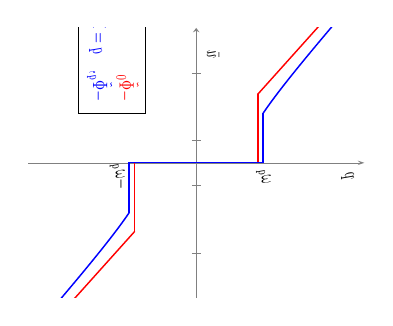
\begin{tikzpicture}[scale=0.5, rotate=90, yscale=-1.5, transform shape]
  \begin{axis}[
    domain=-15:15,
    samples=200,
    axis lines=middle,
    ymax=5,
    ymin=-5,
    xmax=3,
    xmin=-3,
    xtick={-2,-0.5,0,0.5,2},
    ytick=\empty,
    yticklabels={},
    xticklabels={},
    axis line style={gray},
  ]

    \addplot[color=blue, thick, domain=1.108:15 ] {1.2*x+0.7*abs(x)^(-0.5)};
    \addplot[color=blue, thick, domain=-15:-1.108 ] {1.2*x-0.7*abs(x)^(-0.5)};

    \addplot [thick,color=red,mark=.,mark size = 1pt] coordinates {
      (1.527, 1.833) 
      (0, 1.833)
      (0, -1.833)  
      (-1.527, -1.833)
    };

    \addplot [thick,color=red,mark=.,mark size = 1pt] coordinates {
      (0, 1.833)
      (0, -1.833)
    };    

    \addplot[color=red, thick, domain=1.527:15 ] {1.2*x};
    \addplot[color=red, thick, domain=-15:-1.527] {1.2*x};

    \addplot [thick,color=blue,mark=.] coordinates {
      (1.108, 1.994) 
      (0, 1.994)
      (0, -1.994)  
      (-1.108, -1.994)
    };

    \addplot [thick,color=blue,mark=.] coordinates {
      (0, 1.994)
      (0, -1.994)
    };

    \node [draw=black,anchor=center] at (axis cs: 2.4,-2.5) {
      $
      \begin{array}{l}
        {\color{red} -\tilde\Phi_0}\\
        {\color{blue} -\tilde\Phi_q,\quad q=1/2}
      \end{array}
      $
    };

    \node [anchor=center] at (axis cs: -0.3,4.5) {$p$};
    \node [anchor=center] at (axis cs: -0.3,2) {$\omega_q$};
    \node [anchor=center] at (axis cs: -0.3,-2.3) {$-\omega_q$};
    \node [anchor=center] at (axis cs: 2.4,0.5) {$\bar u$};

  \end{axis}
\end{tikzpicture}
\caption{Ilustration of $-\tilde\Phi_q$ compared with the extension of the hard-thresholding operator}
\end{figure}

	Then, we consider the following generalized system 
	
	\begin{subequations}\label{eq:system2.5}
		\begin{align} 
			&	\begin{array}{rll}
				A   y - \tilde u \ni &f, &\hbox{in  } \om, \\
				y=&0, &\hbox{on  }  \Gamma,
			\end{array} \\
			%	
			&\begin{array}{rll}
				A^*   \varphi=& \bar y -y_d, &\hbox{in  } \om, \\
				\varphi=&0, &\hbox{on  }  \Gamma,
			\end{array}\label{eq:statey_2}\\
			&\tilde u (x) = \tilde\Phi_q (\varphi(x)), \quad  \text{a.a. } x \in \om. \label{eq:uPhi.1}
		\end{align} 	
	\end{subequations}
	
	%=====================================================================================
\begin{assumption}\label{as:phi_zero_measure}
    Suppose that $\bar u \in L^2(\om)$ is an optimal control for \eqref{eq:OCP} with associated state $\bar y$ satisfying the state equation \eqref{eq:state} and $\varphi$ satisfying the adjoint equation \eqref{eq:state*}. Then, the set
    $$\om_*=\{x \in \om : |\varphi(x)|=w_q\},$$
    is of measure zero.
\end{assumption}
In practice, this is not a restrictive assumption because the adjoint state is expected to cross the threshold quantity $w_q$ in a set of measure zero.  

 \begin{theorem}\label{t:existence}
		Problem \eqref{eq:system2.5}	admits a unique solution $(y,\varphi) \in H_{0}^{1}(\om) \times H_{0}^{1}(\om)$ with relaxed control $\tilde u = \tilde \Phi_q(\varphi)\subset L^2(\om)$. 
		If, in addition, Assumption \ref{as:phi_zero_measure} holds, then $\bar u = \Phi_q(\varphi)$ is the unique solution to problem \eqref{eq:OCP}.\end{theorem}
	\begin{proof}
		 The proof is analogous to the proof \cite[Section 2.2]{ito-kunisch2014}. However, we consider specifics aspects of the $L^q$ penalizer and $\Phi_q$ defined in \eqref{eq:Phi2}.  For the convenience of the reader, we write down the details. 
		
		As discussed earlier, condition \eqref{eq:1d_fonc} and the monotonicity of $\alpha u + \beta q |u|^{q-1}\sign(u)$ allowed us to define monotone the operator $-\Phi_q$ and its maximal monotone extension $-\tilde\Phi_q$  defined in \eqref{eq:Phi_ext}. This is the main tool for the proof.  
		
Notice that, from \eqref{eq:Phi_ext} and the fact that $u$ and $p$ have opposite signs when $|p|\geq \omega_q$, it holds that   
		
		$$\textcolor{blue}{\left|-\frac{p}{\alpha} - \frac{\beta q}{\alpha} |u|^{q-1}{\sign(\bar u)} \right|= |u| =\frac{|p|}{\alpha}-\frac{\beta q}{\alpha}|u|^{q-1} \leq \frac{|p|}{\alpha}.}$$
		%
		On the other hand, for $w \in L^2(\om)$ we have that $u=\tilde\Phi_q(w)$ belongs to $L^2(\om)$: 
		
		\begin{align*}
			\int_\om u(x)^2 dx =& \int_{|w(x)|\geq \omega_q} \tilde\Phi_q(w(x))^2 \,dx\\		
			=& \int_{|w(x)|\geq  \omega_q} \l|-\frac{w(x)}{\alpha} - \frac{\beta q}{\alpha} |u(x)|^{\textcolor{red}{q-1}}\sign(u(x)) \r|^2 dx \\
			\leq& \int_{|w(x)|>  \omega_q}  \frac{|w(x)|^2}{\alpha^2}  dx+ c^* |\{x\in\om: w(x)=\omega_q\}| \\
			\leq& \int_{|w(x)|>  \omega_q}  \frac{|w(x)|^2}{\alpha^2}  dx+ c^* |\om|<\infty,
			%				    
		\end{align*}
		%
		where $c^*$ is a positive constant, depending on $\jump_q$ and $\omega_q$.
		
		Since the last implies that $\tilde\Phi_q$ is defined from  $L^2(\om)$ into itself, let us consider the generalized system
		
		\begin{equation}\label{eq:monotone_system}
			%
			\l\{
			\begin{array}{lrll}
				&Ay -   \Phi_q(\varphi)  & \ni f,  & \text{ in }  \om,  \\
				&A^*\varphi - y  &= -y_d,  &        \text{ in }   \om,  \\
				& y=\varphi &= 0,  & 	 \text{ on } \ga .
			\end{array}
			\r.
			% 
		\end{equation}
		Let $D(A)=\{v \in H_{0}^{1}(\om): Av \in L^2(\om) \}$ and $D(A^*)=\{v \in H_{0}^{1}(\om): A^*v \in L^2(\om) \}$ the domains of $A$ and $A^*$, respectively, which are densely embeded in $L^2(\om)$. Thus, $A\in \mathcal L(D(A),L^2(\om))$ and therefore $A^*\in \mathcal L(D(A^*),L^2(\om))$ are isomorphisms, see \cite[Section I.4.]{showalter97}; moreover $A$ and $A^*$ are uniformly elliptic by \eqref{eq:uelliptic}.  Then, according to \cite[Proposition 2.6]{ito-kunisch2014}, $AA^*$ is also a maximal monotone operator with domain
		$$D(AA^*)=\{ v \in H_{0}^{1}(\om): A^*v \in D(A)  \}. $$
		Replacing the first equation of \eqref{eq:monotone_system} into the second, we obtain the generalized equation
		\begin{equation}\label{eq:monotone_phi}
			AA^*\varphi -\tilde\Phi(\varphi) \ni f-Ay_d,
		\end{equation}
		provided that $y_d$ belongs to $D(A)$.
		
		Moreover, $AA^* - \tilde\Phi_q(\cdot) $ is maximal monotone satisfying the coercivity property:
		%
		\begin{align}\label{eq:AA*coer}
			( AA^*\varphi -\tilde\Phi_q(\varphi) ,\varphi )_{L^2(\om)}\geq ( AA^*\varphi  ,\varphi )_{L^2(\om)} \geq c_A \norm{\varphi}^2_{H_{0}^{1}(\om)} , \quad \forall \varphi \in D(AA^*).
		\end{align}
		Hence, as in \cite{ito-kunisch2014} we apply \cite[Corollary 2.3]{brezis} concluding that equation \eqref{eq:monotone_phi} has a solution in $H_{0}^{1}(\om)$, denoted by $\varphi$. According to the  second equation in \eqref{eq:monotone_system}, the state is determined by $y=y_d- A^*\varphi$. In this way, $\varphi$ and $y$ satisfy  \eqref{eq:monotone_system}. 
		
		The case $y_d \in L^2(\om)$ is obtained with the procedure from \cite[Proposition 2.6]{ito-kunisch2014}  using the density of $D(A)$ in $L^2(\om)$. 
		
		In addition, from  \eqref{eq:monotone_phi} and \eqref{eq:AA*coer}  we obtain the bound 
		\begin{align}
			c_A\norm{\varphi}_{H_{0}^{1}(\om)} ^2\leq	(AA^*\varphi,\varphi)_{L^2(\om)} \leq & (f-Ay_d,\varphi)_{L^2(\om)},
		\end{align}
		therefore, there exists some $\kappa>0$ such that 
		\begin{equation}
			\norm{\varphi}_{L^2(\om)} \leq\kappa ( \norm{f}_{L^2(\om)} + \norm{y_d}_{L^2(\om)}).\\
		\end{equation}
		The same estimate is true for $y$ by \eqref{eq:statey_2}, i.e. there exists a constant $\kappa>0$ such that
		\begin{equation}
			\norm{y}_{L^2(\om)} \leq\kappa ( \norm{f}_{L^2(\om)} + \norm{y_d}_{L^2(\om)}).\\
		\end{equation}
		Uniqueness follows from the same arguments as in \cite{ito-kunisch2014}.
		
		\subsubsection*{Global solution of \eqref{eq:OCP}} Let us consider $\bar u \in  \tilde\Phi_q (\varphi)$, % =\tilde  \Phi (\varphi) \in L^2(\om)$. 
		together with $\bar y = S \bar u + y_f$ and $\varphi = S(\bar y -y_d) $, satisfying the first-order necessary conditions. Since, by our assumption, the measure of the set $\{x\in \om : |\varphi(x)|=\omega_q \}$ has zero measure, from \eqref{eq:fonc_H}, we have the condition 
		$$ 0 \leq \frac{\alpha}{2}   u(x)^2 + \beta |  u(x)|^q + \varphi (x)  u(x)-\frac{\alpha}{2} \bar u(x)^2 - \beta |\bar u(x)|^q - \varphi (x) \bar u(x), \quad \forall u  \in L^2(\om)$$ 
		holds for almost all $x\in \om$. From this relation, it follows that 
       \begin{equation}\label{eq:diffnonconvex}
           \beta\int_\om |\textcolor{blue}{ u(x)}|^q \, dx - \beta\int_\om |\bar u(x)|^q \, dx \geq \int_\om \frac{\alpha}{2} \bar u(x)^2 - \frac{\alpha}{2}  \textcolor{blue}{u(x)^2}\, dx - \int_\om \varphi(x) ( u(x)-\bar u(x)) \, dx.
       \end{equation}

  Thus, taking into account the differentiable terms of the cost function, we have		
		%%$F'(\bar y,\bar u)[v,z] = (\bar y - y_d, S z) +\alpha(\bar u,v)$; therefore,
		\begin{align}
			J(y,u) - J(\bar y,\bar u) = &(\bar y - y_d, S (u-\bar u))_{L^2(\om)} +\alpha(\bar u,u - \bar u)_{L^2(\om)} + \frac{1}{2}\norm{y -\bar y}_{L^2(\om)}^2   \nonumber\\
			&+ \frac{\alpha}{2}\norm{u -\bar u}_{L^2(\om)}^2+ \beta\int_\om |u(x)|^q dx - \beta\int_\om |\bar u(x)|^q dx\nonumber \\
			=&\int_\om (\alpha \bar u(x) + \varphi (x))(u(x)- \bar u(x)) dx + \frac{\alpha}{2}\norm{u -\bar u}_{L^2(\om)}^2 \nonumber\\
			&+ \frac{1}{2}\norm{y -\bar y}_{L^2(\om)}^2 + \beta\int_\om |u(x)|^q dx - \beta\int_\om |\bar u(x)|^q dx, \nonumber
		\end{align}
where we replace \eqref{eq:diffnonconvex} to get
  \begin{align}
			J(y,u) - J(\bar y,\bar u) \geq &\int_\om (\alpha \bar u(x) + \varphi (x))(u(x)- \bar u(x)) dx + \frac{\alpha}{2}\norm{u -\bar u}_{L^2(\om)}^2 \nonumber\\
			&+ \frac{1}{2}\norm{y -\bar y}_{L^2(\om)}^2 + \int_\om \frac{\alpha}{2} \bar u(x)^2 - \frac{\alpha}{2}   u(x)^2 dx \nonumber \\
   &- \int_\om \varphi(x) ( u(x)-\bar u(x)) \, dx \nonumber \\
   = &  \frac{\alpha}{2}\norm{u -\bar u}_{L^2(\om)}^2 + \frac{1}{2}\norm{y -\bar y}_{L^2(\om)}^2  \nonumber\\
   &+  \int_\om  \alpha \bar u(x)(u(x)- \bar u(x) ) +\frac{\alpha}{2} \bar u(x)^2 - \frac{\alpha}{2} u(x)^2 dx \nonumber \\
  =& \frac{1}{2}\norm{y -\bar y}_{L^2(\om)}^2  \geq 0. \nonumber
		\end{align}
% 		We analyze the last integrals in \eqref{eq:J-J1}  separately, in the following sets: $\om^*:= \{x\in \om : |\varphi(x)|=\omega_q \}$, $\om_{\omega_q}:= \{x\in \om : |\varphi(x)|>\omega_q \}$ and $\om_0:= \{x\in \om : |\varphi(x)|<\omega_q \}$. 
% 		%Moreover, its associated state is denoted by $\bar y$, which together with $\varphi$ solve system \eqref{eq:system1}.
% 		%
% 		%From \eqref{eq:J-J1}, and having in mind that $|\om^*|=0$ we deduce
		
% 		For almost all $x\in \om_{\omega_q}$, we have that $\bar u(x)\not =0$ and satisfy \eqref{eq:fonc_ell} with $p=\varphi(x)$. Then, we get 
% 		\begin{align}
% 			\int_{\om_{\omega_q}} &(\alpha \bar u(x) + \varphi (x))(u(x)- \bar u(x)) dx  + \beta\int_{\om_{\omega_q}} |u(x)|^q dx - \beta\int_{\om_{\omega_q}} |\bar u(x)|^q dx  \nonumber \\
% 			=& \beta\int_{\om_{\omega_q}}  |u(x)|^q-   |\bar u(x)|^q  -  q |\bar u(x)|^{q-1}\sign(\bar u(x))(u(x)- \bar u(x)) dx .\nonumber 
% 			%
% 			%=& \int_{\om_1^*} \beta |u(x)|^q- \beta |\bar u(x)|^q  -\beta q |\bar u(x)|^{q-1}(u(x)- \bar u(x)) dx \nonumber \\
% 		\end{align}
% 		%
% 		Due to the properties of the function $u\mapsto\alpha u+\beta q|u|^{q-1}\sign(u)$ analyzed previously in Theorem 1, we have that for almost all $x\in \om$ such that $|\varphi(x)|>\omega_q$, $|\bar u(x)|>\jump_q$. Therefore, using a Taylor expansion around $|\bar u(x)|>\jump_q$, %for $t\in (0,1)$ and $u_t(x):=\bar u(x) + t(u(x)-\bar u(x))$, for almost all $x \in \om_{\omega_q}$; 
%   we have,
% %
%   %  \begin{align*} \int_{\om_{\omega_q}} &\beta |u(x)|^q- \beta |\bar u(x)|^q  -\beta q |\bar u(x)|^{q-1}\sign(\bar u(x))(u(x)- \bar u(x)) dx  \\
%   %  = &\int_{\om_{\omega_q}}  \frac{\beta}{2} q (q-1) \Big( \int_0^1 | u_t(x)|^{q-2} \sign(u_t(x)) dt \Big) (u(x)-\bar u(x))^2 \, dx \\ 
%   %  \geq &- \frac{\beta}{2} q (1-q) \int_{\om_{\omega_q} \cap \{x\in \om: u_t(x) \geq 0 \}} \int_0^1 | u_t(x)|^{q-2}  dt (u(x)-\bar u(x))^2 \, dx
%   %  \end{align*}
  
%   % such that the higher order term $o(|u(x)- \bar u(x)|^2)$ satisfies
%   %  \begin{align*} 
%   %  o(|u(x)- \bar u(x)|^2) =& - q (q-1) \int_0^1 | \bar u(x) + t(u(x)-\bar u(x))|^{q-2} (u(x)-\bar u(x))^2 dt \\
%   %  =& q (1-q) \Big(\int_0^1 | \bar u(x) + t(u(x)-\bar u(x))|^{q-2} dt\Big) (u(x)-\bar u(x))^2 \geq 0,
%   %  \end{align*}
%  then, it follows that
% 		\begin{align}
%   \int_{\om_{\omega_q}} &\beta |u(x)|^q- \beta |\bar u(x)|^q  -\beta q |\bar u(x)|^{q-1}\sign(\bar u(x))(u(x)- \bar u(x)) dx\nonumber\\
% 			=& \int_{\om_{\omega_q}} \frac{\beta}{2}q(q-1)|\bar u(x)|^{q-2} (u(x)- \bar u(x))^2 + o(|u(x)- \bar u(x)|^2) dx \nonumber\\
% 			\geq & \int_{\om_{\omega_q}} \frac{\beta}{2}q(q-1){\jump_q}^{q-2} (u(x)- \bar u(x))^2 dx  + o(\norm{}_{L^2()}) \nonumber \\
% 			= & -q\frac{\alpha}{4}\int_{\om_{\omega_q}} (u(x)- \bar u(x))^2 dx>-q\frac{\alpha}{2}\int_{\om_{\omega_q}} (u(x)- \bar u(x))^2 dx + o(|u(x)- \bar u(x)|^2) . \label{eq:om1} 
% 		\end{align}
% Then, there exist a neighborhood of $\bar u(x)$		
% 		On the other hand, for almost all $x\in\om_0$, we have that $\bar u(x) =0$ solves \eqref{eq:1dlq} with $p=\varphi(x)$, therefore 
% 		\begin{align}
% 			\int_{\om_0} &(\alpha \bar u(x) + \varphi (x))(u(x)- \bar u(x)) dx  + \beta\int_{\om_0} |u(x)|^q dx - \beta\int_{\om_0} |\bar u(x)|^q dx  \nonumber \\
% 			=&\int_{\om_0}\varphi (x) u(x) +\beta |u(x)|^q + \frac{\alpha}{2}u(x)^2 dx -  \int_{\om_0}\frac{\alpha}{2}u(x)^2 dx  \nonumber \\
% 			\geq & -  \int_{\om_0}\frac{\alpha}{2}u(x)^2 dx. \label{eq:om2}
% 		\end{align}
% 		By replacing  \eqref{eq:om1} and \eqref{eq:om2} in \eqref{eq:J-J1} and taking into account that $\om^*$ has zero measure, we arrive to the inequality 
% 		\begin{align}
% 			J(y,u) - J(\bar y,\bar u) =&  \frac{\alpha}{2}\norm{u -\bar u}_{L^2(\om)}^2
% 			+ \frac{1}{2}\norm{y -\bar y}_{L^2(\om)}^2 \nonumber \\
% 			&-q\frac{\alpha}{2}\int_{\om_{\omega_q}} (u(x)- \bar u(x))^2 dx + o(\norm{u -\bar u}_{L^2(\om)}^2) -  \int_{\om_0}\frac{\alpha}{2}u(x)^2 dx \nonumber \\
% 			&=(1-q)\frac{\alpha}{2}\int_{\om_{\omega_q}} (u(x)- \bar u(x))^2 dx +  \frac{1}{2}\norm{y -\bar y}_{L^2(\om)}^2\ \geq 0 \nonumber
% 			\label{eq:J-J12} 
% 		\end{align}
		Then, $\bar u$ is a global minimum.
	\end{proof}

%\begin{lemma}\label{l:biconjugate}
%    Let us consider the penalty integrand of the cost functional of $(P_\lambda)$, given by the function $h(t)=\frac{\alpha}{2}|t|^2+\beta |t|^q$ defined for all $t\in \mathbb{R}$, and let $q\in ]0,1[$. Then, the function $\widehat{h}:\mathbb{R}\to \mathbb{R}$ defined by
%    %
%    \begin{equation}\label{biconjugate}
%       \widehat{h}(t)=\begin{cases}
%            h(t),&|t|\ge t^*,\\
%            r^*|t|,&|t|<t^*,
%        \end{cases}
%    \end{equation}
%where
%\[
%    t^*=\left(\frac{2\beta}{\alpha}(1-q)\right)^{\frac{1}{2-q}},
%\]
%and $r^*=\alpha t^*+\beta q(t^*)^{q-1}$, corresponds to the biconjugate of $h$. In addition, its convex subdifferential corresponds to
%   \begin{equation}\label{sub_biconjugate}
%       \partial \widehat{h}(t)=\begin{cases}
%           \alpha t+\beta q |t|^{q-1}\sign(t), &|t|\ge t^*,\\                     
%           r^*\sign(t), &|t|<t^*, t\ne 0,\\
%           \eta\in [-r^*,r^*], &t=0.
%       \end{cases}
%   \end{equation}
%\end{lemma}

\begin{remark}\label{r:convexification}
	     Theorem \ref{t:monotone_phi} provides a functional relation between the optimal control $\bar u$ and the adjoint state $\varphi$. Moreover, from Theorem \ref{t:existence}, the relation \eqref{eq:system2_gradeq} and under Assumption \ref{as:phi_zero_measure}, we have
      \begin{equation}
      \Omega_{\jump_q}=\{x: |\bar u(x)| > \jump_q\} = \{x: |\varphi(x)| >\omega_q \} \label{eq:Omega_jump_set}
      \end{equation}

Additionally, let us observe that the system \eqref{eq:monotone_system} is, in fact, an optimality system associated with a convex optimal control problem, provided that the set $\om^* = \{x \in \om: |\varphi(x)|=\omega_q \}$ has zero measure. 
Indeed, let us consider the real convex function	
\begin{equation}
	\phi_q(u)= 
\begin{cases}
		 \frac{\alpha}{2} u^2 + \beta |u|^q,	& \text{ if } |u| > \jump_q, \\
		 \omega_q |u|,	& \text{ if } |u|\leq \jump_q,
\end{cases}
\label{eq:phi}
\end{equation} 

whose subdifferential is given by
 
 $$ \partial \phi_q(u)= 
\begin{cases}
		 \{\alpha u + \beta q|u|^{q-1}\sign(u) \},	& \text{ if } |u|> \jump_q, \\
		 \{ \omega_q \sign(u) \},	& \text{ if } 0<| u|\leq  \jump_q, \\
		 [-\omega_q,\omega_q] & \text{ if }  \bar u = 0.
\end{cases}
 $$
 Thanks to the definition of $\phi_q$, under Assumption \ref{as:phi_zero_measure}, we characterize the control $\bar u(x)= -\tilde \Phi(\varphi)$ as a solution of the optimal control problem: 
 \begin{equation}
		\tag{$\tilde P$} \label{eq:OCP_conv}
		\begin{cases}
			\displaystyle\min_{(y,u)} \tilde J(y,u) := \frac12 \norm{y-y_d}^2_{L^2(\om)} + \int_\om \phi_q (u(x)) dx \\
			\hbox{ subject to: }\\
			\hspace{40pt}\begin{array}{rll}
				A y(x) =&u(x) + f(x), &\hbox{in  } \om, \\
				y(x)=&0, &\hbox{on  }  \Gamma,
				%\dfrac{\partial y}{\partial \vec{n}}=0&\hbox{sobre  } \Gamma. %, $\gamma= 1e4$,
			\end{array}
			%			\\
			%			\hspace{45pt} u \in L^2(\om),
		\end{cases}
	\end{equation}
 whose optimality conditions are given by \eqref{eq:monotone_system}. To see this, we apply Fermat's principle to the convex functional $\tilde J(S\cdot,\cdot)$; i.e., $0 \in \partial \tilde J(S\cdot,\cdot) (\bar u)$. This fact was also pointed out in \cite{ito-kunisch2014} in the case of the $L^0$-pseudonorm penalizer.
Furthermore, we notice that  for a fixed $q\in (0,1)$ and all $u\in \reals$, the function $\phi_{q}(u)$ satisfies the relation
    \begin{equation}\label{eq:remark2}
        \phi_q(u) \ge \frac{\alpha}{2}|u|^2.
    \end{equation}
Indeed, when $u=0$, the relation holds trivially. Now, from the definition of $\phi_q$ \eqref{eq:phi}, if $|u|>\jump_q$  it is clear that
    \[
    \phi_q(u)=\frac{\alpha}{2}|u|^2+\beta|u|^q \ge \frac{\alpha}{2}|u|^2.
    \]
    On the other hand, if $|u|\le\jump_q$, then $\alpha\jump_q\ge\alpha|u|$. Since $bq(\jump_q)^{q-1}>0$, we have that $\alpha\jump_q+bq(\jump_q)^{q-1}>\alpha\jump_q\ge\alpha|u|$. Multiplying both sides of the last inequality by $|u|$, and using \eqref{eq:phi} on $[-\jump_q,\jump_q]$ we get that
    \[
        \phi_q(t)>\alpha|t|^2\ge\frac{\alpha}{2}|t|^2.
    \]  
    Finally, observe, that  the function
    \[
    d_{q}(u,v):=\int_{\om}\phi_q(u(x)-v(x))\; dx,
    \]
    defined for all $u,v\in L^2(\om)$, is a metric on $L^2(\om)$. This fact can be checked easily from the non-negativeness of $\phi_q$ plus the fact that, for any $a,b\ge 0$ and $q\in(0,1)$, we have $(a+b)^q\le a^q+b^q$.
\end{remark}    


 
\subsection{Incorporating box-constraints on the controls}
Let us briefly discuss the modifications of the previous results to incorporate control constraints. Let \(u_a\) and \(u_b\) be real numbers such that \(u_a \leq 0 \leq u_b\) with \(u_a \ne u_b\). We define the set \(U = \{t \in \mathbb{R} : u_a \leq t \leq u_b\}\),  and  
\begin{equation}\label{eq:Uad}  u \in U_{ad}= \{ v \in L^2(\om): v(x) \in U, \, \text{ for almost all }x\in \om \}. \end{equation}
Then, the maximum principle is applied to the extended Hamiltonian:
\begin{equation} 
\mathcal H(x,y,u,p)= \frac{1}{2}|y-y_d(x)|^2 + \frac{\alpha}{2}u^2 + \beta |u|^q + pu + \mathcal{I}_{U}(u),	\nonumber
\end{equation}
which leads to the optimization	problem \eqref{eq:1dlq}, restricted to the interval $[u_a,u_b]$. Therefore, its solution can be expressed in terms of the projection on the interval $[u_a,u_b]$; that is:
\begin{equation}\label{eq:1dlqc}
		\bar u \displaystyle\in  \argmin_{u\in [u_a,u_b]} \left\{ \frac{\alpha}{2}u^2+\beta |u|^q + pu \right\},
	\end{equation}

We have learned from the unconstrained case that $|\bar u(x)|>\jump_q>0$ or $\bar u (x)=0$. Therefore, for simplicity, we further assume that $u_a < - \jump_q<0<\jump_q<u_b$. Therefore, the solution $\bar u $ is characterized by 
\begin{equation}\label{eq:Phi2_c}
			%
	\bar u=		\mathcal{P}_{[u_a,u_b]}(\Phi_q (p)) =	
			%
			\begin{cases}
			u_a, &  \text{ if } -p\leq  p_a, \\
			u_b, &  \text{ if } -p\geq  p_b, \\
				-\frac{p}{\alpha}-\frac{\beta}{\alpha} q |\bar u|^{q-1}\sign (\bar u), & \text{ if } \omega_q<|p|,\,  \text{ and } p_a<-p<p_b  , \\
				0,                         &	\text{ otherwise.}
			\end{cases}
\end{equation}
where $p_a : = \alpha u_a -  \beta q  |u_a|^{q-1}<0$	 and $p_b= \alpha u_b +  \beta q  |u_b|^{q-1}>0$. 

It is clear that  $-\mathcal{P}_{[u_a,u_b]}(\Phi_q (p))	$ is also a monotone operator. The projection applied in \eqref{eq:Phi2_c} truncates $-\Phi(x)$ to the interval $[u_a,u_b]$; hence, $- \mathcal{P}_{[u_a,u_b]}(\tilde\Phi_q (p))$ is also maximal monotone. Therefore, Theorem \ref{t:existence} is also valid when optimal control problem includes box-constraints of the form \eqref{eq:Uad}. 

The optimality system for the box-constrained case reads: let $\bar u$ be an optimal control for problem $(P)$ with control constraints \eqref{eq:Uad}; then, there exist $\bar y \in H_{0}^{1}(\om)$ and $\varphi \in \rm{H}_0^2(\om)$ \textcolor{red}{Está bien la regularidad de $\varphi$?} such that the following system is satisfyed:

\begin{subequations}\label{eq:system_box}
		\begin{align} 
			&	\begin{array}{rll}
				A \bar y=& \bar u + f, &\hbox{in  } \om, \\
				\bar y=&0, &\hbox{on  }  \Gamma,
			\end{array} \\
			%	
			&\begin{array}{rll}
				A^*   \varphi=& \bar y -y_d, &\hbox{in  } \om, \\
				\varphi=&0, &\hbox{on  }  \Gamma,
			\end{array}\\
			& \alpha \bar u (x) + \beta q |\bar u(x)|^{q-1} \sign(\bar u(x)) + \varphi(x)  = 0, \\
			& \quad a.a. \, x \in \{x: |\varphi(x)|>\omega_q \text{ and }  p_a<-\varphi(x)<p_b \},\nonumber\\
			& \bar u(x) =0, \quad \text{a.a. }  \, x \in \{x: \,  |\varphi(x)| \leq \omega_q\}, \\
			& \bar u(x) = u_a, \quad \text{a.a. } x \in \{x: -\varphi(x) \leq p_a\}, \\
			& \bar u(x) = u_b, \quad \text{a.a. } x \in \{x: -\varphi(x) \geq p_b\}.
		\end{align} 	
	\end{subequations}
	
As in the unconstrained case, this system might not be solvable if the measure of the set $\{x\in\om:|\varphi(x)|=\omega_q\}$ is not null. Moreover, the solution $\bar u \in U_{ad}$ is also the solution to the constrained convexified optimal control problem:

 \begin{equation}
		\tag{$\tilde P_C$} \label{eq:OCP_conv_c}
		\begin{cases}
			\displaystyle\min_{(y,u)} \tilde J(y,u) := \frac12 \norm{y-y_d}^2_{L^2(\om)} + \int_\om \phi_q (u(x)) \; dx \\
			\hbox{ subject to: }\\
			\hspace{40pt}\begin{array}{rll}
				A y(x) =&u(x) + f(x), &\hbox{in  } \om, \\
				y(x)=&0, &\hbox{on  }  \Gamma,
				%\dfrac{\partial y}{\partial \vec{n}}=0&\hbox{sobre  } \Gamma. %, $\gamma= 1e4$,
			\end{array}
						\\
						\hspace{45pt} u \in U_{ad}.
		\end{cases}
	\end{equation}


\subsection{Convex relaxation of \eqref{eq:OCP}} There is no guarantee that problem \eqref{eq:OCP} admits a solution. A usual procedure to deal with problems involving nonconvex penalizers is to consider a partial convexification, consisting of replacing the nonconvex penalizer by its convex envelope, which is viewed as the ``best'' lower-semicontinuous convex minorant, also known as $\Gamma$-regularization.

For the cost function of \eqref{eq:OCP}, we consider the convex envelope of $\phi_q(t) = \dfrac{\alpha}{2} |t|^2 + \beta |t|^q$; therefore $\phi_q$ is replaced by its biconjugate denoted by $\phi_q^{**}$. It is straightforward to see that
$$\phi_q^{**}(t) =
\begin{cases}
    \phi_q(t), & \text{if} \, |t|\ge \jump_q,\\
    \omega_q|t|,   & \text{otherwise}.
\end{cases}
$$
where the quantities $\jump_q$ and $\omega_q$ are defined by
\begin{equation}\label{eq:jump_bound}
\jump_q :=\;
\l(2(1-q) \frac{\beta}{\alpha} \r)^{\frac{1}{2-q}}
\quad \text{ and } \quad
\omega_q :=\; \alpha \frac{2 - q}{2 - 2q}\,
\jump_q.
\end{equation} 
In particular, $\jump_q$ measures the length of the jump discontinuity of the optimal control, which depends nonlinearly on $q$.
%

Thus, we formulate the convex optimal control problem
\begin{equation}
		\tag{$\tilde P$} \label{eq:OCP_conv}
		\begin{cases}
			\displaystyle\min_{(y,u)} \tilde J(y,u) := \frac12 \norm{y-y_d}^2_{L^2(\om)} + \int_\om \phi^{**}_q (u(x)) dx \\
			\hbox{ subject to: }\\
			\hspace{40pt}\begin{array}{rll}
				A y(x) =&u(x) + f(x), &\hbox{in  } \om, \\
				y(x)=&0, &\hbox{on  }  \Gamma,
				%\dfrac{\partial y}{\partial \vec{n}}=0&\hbox{sobre  } \Gamma. %, $\gamma= 1e4$,
			\end{array}
			%			\\
			%			\hspace{45pt} u \in L^2(\om),
		\end{cases}   
	\end{equation}

Since $\phi_q^{**}\geq ct^2$ for some positive constant $c$, then any minimizing sequence is bounded in $L^2(\om)$. Therefore, the direct method of the calculus of variations implies that \eqref{eq:OCP_conv} has a solution in $L^2(\om)$. However, the lack of strict convexity of $\tilde J$ prevents its uniqueness.

\subsection{Optimality conditions for \eqref{eq:OCP_conv}} The adjoint state is an essential tool to represent optimality conditions. Given an optimal control $\tilde u \in L^2(\om)$ for \eqref{eq:OCP_conv} with adjoint state $\tilde \varphi$ solution of the variational problem \eqref{eq:costate} with $y=\tilde y = S \tilde u +y_f$, then $\tilde\varphi$ corresponds to the derivative at $\tilde u$ of the function $F(u) = \frac12 \norm{Su-y_d}^2_{L^2(\om)}$ in $L^2(\om)$.

Let $\tilde j(u)= \int_\om \phi_q^{**}(u(x)) dx$ and let $\partial \tilde j$ be its subdifferential. If $\tilde{u}$ is an optimal control for \eqref{eq:OCP_conv} then by the Fermat’s principle the first-order optimality condition is
$0 \in \tilde{\varphi} \;+\partial \tilde{j} (\tilde{u})$, which we aim to solve for $\tilde{u}$. Proceeding formally, notice that $\tilde j$ is proper and weakly lower semicontinuous. Therefore, it follows that $\partial \tilde j$ is maximally monotone and its (negative) inverse $\tilde\Phi_q :=-(\partial \tilde j)^{-1}$ is defined as a multifunction. Thus, we can write
$$ \tilde u \in \tilde \Phi_q(\tilde \varphi).$$
The operator $\tilde \Phi_q: L^2(\om) \rightrightarrows L^2(\om) $, was introduced in \cite{ito-kunisch2014} for $q=0$ ($L^0$-pseudonorm) through the Pontryagin's maximum principle and using the proximity operator of the $\ell_0$ pseudonorm (known in finite dimensions as hard-thresholding). An analogous operator $\tilde \Phi_q$, for $q\in (0,1)$, can be defined using the proximity mapping of the function $\reals \ni t \mapsto |t|^q$, see \eqref{eq:prox_lq} below. In contrast to the hard-thresholding for $q=0$, the corresponding mapping for $q \in (0,1)$ is implicitly defined.  See \cite{bredies03} for the definition of this mapping in finite dimensions. 

Thus, if $\varphi$ is the adjoint state associated with a control $u$ by equation \eqref{eq:costate}, we denote by $\tilde \Phi_q=-(\partial \tilde j)^{-1}:  L^2(\om) \rightrightarrows L^2(\om)$ which is given by 
%
\begin{equation}\label{eq:Phi_ext}
		%
		\tilde\Phi_q (\varphi)  =	
		%
		\begin{cases}
			-\frac{\varphi}{\alpha}-\frac{\beta}{\alpha} q |u|^{q-1}\sign (u), & \text{ if } |\varphi|>\omega_q, \\
			0,                          &	 \text{ if } |\varphi|<\omega_q, \\
			[-\jump_q, 0] ,                         &	 \text{ if } \varphi=\omega_q,\\
			[0,\jump_q],                         &	 \text{ if } \varphi=-\omega_q.
		\end{cases}
	\end{equation}
    where $\jump_q$ and $\omega_q$ where defined in \eqref{eq:jump_bound}. Figure (1.A) illustrates operators $-\tilde\Phi_q$ for $0\leq q<1$ and $-\tilde\Phi_0$. 

We use $\tilde \Phi_q$ to write the associated optimality system. Let $\tilde u \in L^2(\om)$ be an optimal control for \eqref{eq:OCP_conv}, there exist $\tilde y$ and $\tilde \varphi$ in $H_0^1(\om)$ that satisfy
\begin{subequations}\label{eq:system2.5}
		\begin{align} 
			&	\begin{array}{rll}
				A   \tilde y  =& \tilde u + f, &\hbox{in  } \om, \\
				\tilde y=&0, &\hbox{on  }  \Gamma,
			\end{array} \\
			%	
			&\begin{array}{rll}
				A^*   \tilde\varphi=& \tilde y -y_d, &\hbox{in  } \om, \\
				\tilde \varphi=&0, &\hbox{on  }  \Gamma,
			\end{array}\label{eq:statey_2}\\
			&\tilde u (x) \in \tilde\Phi_q (\tilde\varphi(x)), \quad  \text{a.a. } x \in \om. \label{eq:uPhi.1}
		\end{align} 	
	\end{subequations}


